%%%%%%%%%%%%%%%%%%%%%%%%%%%%%%%%%%%%%%%%%%%%%%%%%%%%%%%%%%%%%%%%%%%%%%
%%%%%%%%%  TEMPLATE IEEE PARA ENTREGA DEL ARTÍCULO FINAL DE  %%%%%%%%% 
%%%% PRÁCTICA DE INGENIERÍA ELECTRÓNICA DE LA UNIVERSIDAD CENTRAL %%%%
%%%%%%%%%%%%%%%%%%%%%%%%    BOGOTÁ, COLOMBIA    %%%%%%%%%%%%%%%%%%%%%%
%%%%%%%%%%%%%%%%%%%%%%%%%%%%%%%%%%%%%%%%%%%%%%%%%%
%%%%   AUTOR: SERGIO ANDRÉS CHAPARRO MORENO   %%%%
%%%%%%%%%%%%%%%%%%%%%%%%%%%%%%%%%%%%%%%%%%%%%%%%%%
%%%%%%%%%%%%%  VERSIÓN 1.0-ENE 2017  %%%%%%%%%%%%%
%%%%%%%%%%%%%%%%%%%%%%%%%%%%%%%%%%%%%%%%%%%%%%%%%%
\documentclass[journal]{IEEEtran}
\IEEEoverridecommandlockouts
%%%%%%%%%%%%%%%%%%%%%%%%%%%%%%%%%%%%%%
%%%%%%%% PRINCIPALES PAQUETES %%%%%%%%
%%%%%%%%%%%%%%%%%%%%%%%%%%%%%%%%%%%%%%
\usepackage{fancyhdr}
\usepackage{graphicx}
\usepackage[utf8]{inputenc}
\usepackage{color}
\usepackage{hyperref}
\usepackage{wrapfig}
\usepackage{array}
\usepackage{multirow}
\usepackage{adjustbox}
\usepackage{nccmath}
%\usepackage{anysize}
\usepackage{pgfplots}
\usepgfplotslibrary{external}
\tikzexternalize
\usepackage{subfigure}
\usepackage{amsfonts,latexsym} % para tener disponibilidad de diversos simbolos
\usepackage{enumerate}
\usepackage{booktabs}
\usepackage{float}
\usepackage{threeparttable}
\usepackage{array,colortbl}
\usepackage{ifpdf}
\usepackage{rotating}
\usepackage{cite}
\usepackage{stfloats}
\usepackage{url}
\usepackage{listings}

\newcolumntype{P}[1]{>{\centering\arraybackslash}p{#1}} 
\newcommand{\tabitem}{~~\llap{\textbullet}~~}
\newcommand{\ctt}{\centering\scriptsize\textbf} %%\ctt abrevia el comando \centering\scriptsize\textbf
\newcommand{\dtt}{\scriptsize\textbf} 
\renewcommand\IEEEkeywordsname{Palabras clave}


% correct bad hyphenation here
\hyphenation{op-tical net-works semi-conduc-tor} 

\graphicspath{ {Figs/} } 



\newcommand{\MYhead}{\smash{\scriptsize
\hfil\parbox[t][\height][t]{\textwidth}{\centering
\begin{picture}(0,0) \put(-0,-15){
\includegraphics[width=30mm]{cued}} \end{picture} \hspace{6.5cm}
University of Cambridge \hspace{5.3cm} Version 1.0\\
\hspace{6.6cm} Department of Engineering \hspace{5cm} Date 2018-11\\
\underline{\hspace{ \textwidth}}}\hfil\hbox{}}}
\makeatletter
% normal pages
\def\ps@headings{%
\def\@oddhead{\MYhead}%
\def\@evenhead{\MYhead}}%
% title page
\def\ps@IEEEtitlepagestyle{%
\def\@oddhead{\MYhead}%
\def\@evenhead{\MYhead}}%
\makeatother
% make changes take effect
\pagestyle{headings}
% adjust as needed
\addtolength{\footskip}{0\baselineskip}
\addtolength{\textheight}{-1\baselineskip}
\usepackage{nomencl}
\makenomenclature
\pgfplotsset{compat=1.9}
\begin{document}

\title{3E3 Coursework: Pharmaceutical Licensing Contract Evaluation}

\author{Tom Xiaoding Lu\\
				\textit{xl402@cam.ac.uk}\\
				Pembroke College\\% stops a space
} %\thanks anexa una nota a pie de página donde se puede colocar alguna información sobre la naturaleza del documento.
%%%%%%%%%%%%%%%%%%%%%%%%%%%
%\thanks{El presente documento corresponde al articulo final del proyecto de práctica de ingeniería electrónica 3 presentado en la Universidad Central durante el periodo 2017-1.}
% Comando que indica la generación del título
\maketitle

\begin{abstract}
The project aims to investigate the licensing contract between the pharmaceutical company PHARMA, a potential licensee entering a contract with BIO regarding the development and marketing of the drug ND.\\ Decision and sensitivity analysis are carried out in evaluation the EMV for the respective companies.
\end{abstract}

\mbox{}
\nomenclature{Succ.}{Successful}
\nomenclature{Count.}{Continue}
\nomenclature{Term.}{Terminate}
\nomenclature{Abd.}{Abandon}
\nomenclature{DEP}{Anti-depression drug}
\nomenclature{WL}{Weight Loss drug}
\nomenclature{EMV}{Expected monetary value}
\nomenclature{EVPI}{Expected value of perfect information}
\printnomenclature

\section{Introduction}
\IEEEPARstart{D}{ue} to uncertainty and asymmetric information, company shares and investment in drug discoveries differ significantly in valuation and risk assessment \cite{bioe}. As company shares are frequently traded, damage is controlled at low-transaction costs. Whereas selling an under performing drug is costly, and there is no list of historic prices for that specific drug to allow buyer to estimate the current value. Furthermore, the asymmetric information problem arises because the buyer cannot verify that the seller is telling the truth.\\
Licensing contracts have features that allow the parties to spread cash transfer over the life cycle of the drug making it a suitable contract between both the large pharmaceutical companies and bio-entrepreneurs. This report aims to investigate the licensing contract between PHARMA (licensee) and BIO (licensor) regarding the development and marketing of the drug ND. The drug was originally developed to treat depression, later discovered it also blocks the receptor that causes hunger. At the time of offer, ND is under pre-clinical development ready to enter the three phase clinical approval process. The details of the agreement can be found in \cite{coursework}, under the licensing contract, a decision tree of the FDA approval process is made, from which conclusions on whether PHARMA should bid under different conditions is made. The EMV of licensing agreement to BIO assuming 5\% royalty is calculated, sensitivity analysis is made on launching cost for the weight loss program and EVPI for phases I and II of the FDA approval process is made.
\section{Decision Analysis}	
\subsection{FDA Approval Analysis and Advice To Licensee}
Figure \ref{pharma_tree} shows the decision tree for all stages of the FDA approval process, note all decision trees adopt the nomenclature described above. Numbers highlighted in blue denote the probability of arriving at the state indicated. All monetary values have denomination one million. The decision tree is drawn from the policy table extracted from the project brief shown in section \ref{sec:pol}.
\begin{figure}
\centering 
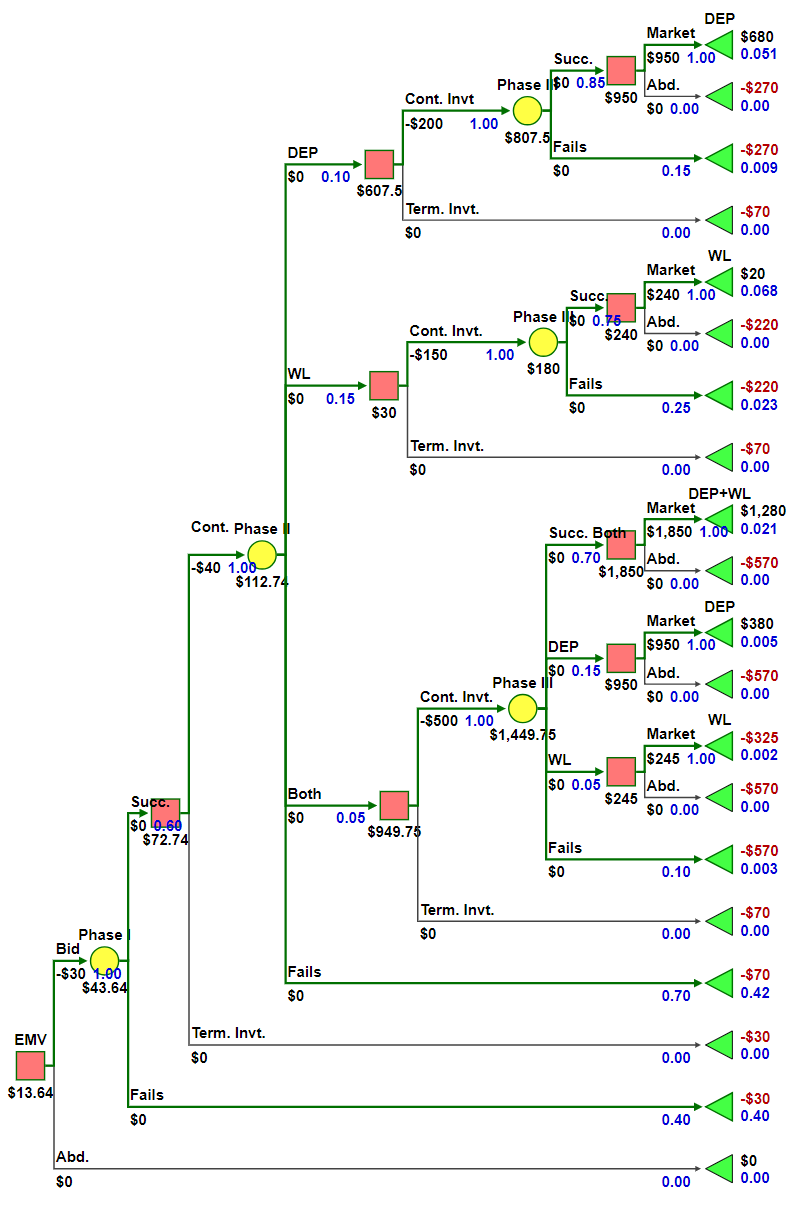
\includegraphics[width = 1.\linewidth]{pharma_tree}
\caption{PHARMA FDA Approval Decision Tree 0\% Royalty} 
\label{pharma_tree} 
\end{figure}
PHARMA needs to decide whether to enter a license contract with BIO. From the decision tree shown in figure \ref{pharma_tree}, the EMV under 0\% post launch royalty is \$13.64M. The value decreases down to \$6.78M under 5\% royalty. The sensitivity analysis of the effect of royalty on the EMV of PHARMA and BIO is shown in figure \ref{fig:loys}. Therefore, bidding for ND is a prudent investment for PHARMA as long as the royalty is kept below 10\%, the bidding price under 0\% and 5\% royalty should be below their EMV values respectively. However, whether or not PHARMA deems the EMV under these royalties over the course of 7 years (length it takes to develope and sell the product until the patent expires) will require taking into account of PHARMA's portfolio which is unknown from the project brief.
\begin{figure}[H]
    \centering
    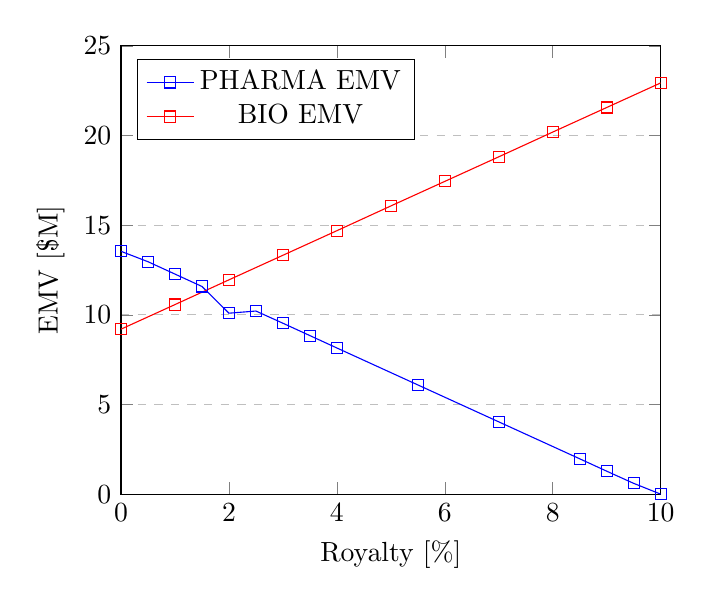
\begin{tikzpicture}
\begin{axis}[
    xlabel={Royalty [\%]},
    ylabel={EMV [\$M]},
    xmin=0, xmax=10,
    ymin=0, ymax=25,
    xtick={0,2,4,6,8,10},
    ytick={0,5,10,15,20,25},
    legend pos=north west,
    ymajorgrids=true,
    grid style=dashed,
]
\addplot[
    color=blue,
    mark=square,
    ]
    coordinates {
    (0,13.54)(0.5,12.96)(1,12.27)(1.5,11.58)(2,10.09)(2.5,10.21)(3,9.53)(3.5, 8.84)(4,8.15)(5.5,6.09)(7,4.03)(8.5,1.97)(9,1.28)(9.5,0.6)(10,0)
    };
\addplot[
    color=red,
    mark=square,
    ]
    coordinates {
    (0,9.2)(1,10.57)(2,11.95)(3,13.32)(4,14.69)(5,16.07)(6,17.44)(7, 18.81)(8,20.19)(9,21.56)(10,22.93)
    };
    \legend{PHARMA EMV, BIO EMV}
\end{axis}
\end{tikzpicture}
    \caption{Loyalty Sensitivity Analysis}
    \label{fig:loys}
\end{figure}


\subsection{Expected Value of Licensing Agreement}
As shown in figure \ref{fig:loys}, the expected value of the licensing agreement to BIO is the EMV from the decision tree (shown in the appendix), under 0\% royalty, BIO's EMV is \$9.20M, although this value is 48.3\% smaller than the EMV of PHARMA, the minimum amount that BIO makes is \$5M and for PHARMA is -\$570M, therefore BIO, having failed to get FDA approval on their latest product is more risk averse hence should prefer the licensing contract over funding its own clinical approval process.
\subsection{Analysis Under Change of Launching Costs}
Sensitivity analysis is also conducted on the cost of launching ND for weight loss the result is shown in figure \ref{fig:wls}, PHARMA suffers a loss in EMV due to abandoning entering Phase III once the result from Phase II shows the drug is only effective for weight loss, its EMV drops from \$13.64M at \$100M marketing cost down to \$10.73M at \$225M marketing cost. BIO also suffers the consequence of higher marketing cost as PHARMA chooses not to further pursuit marketing the product after phase II, its EMV drops down to \$8.3M at 0\% royalty and \$14.02M at 5\% royalty (effectively removing the decision node for WL after Phase II.
\begin{figure}[H]
    \centering
    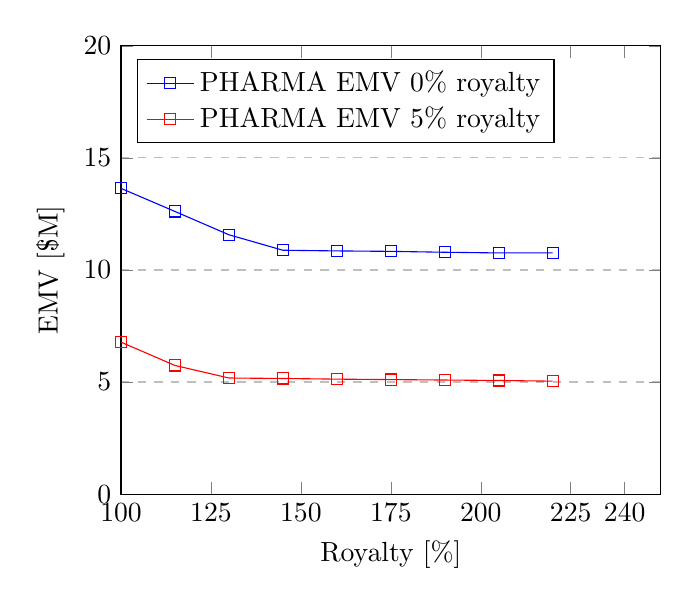
\begin{tikzpicture}
\begin{axis}[
    xlabel={Royalty [\%]},
    ylabel={EMV [\$M]},
    xmin=100, xmax=250,
    ymin=0, ymax=20,
    xtick={100,125,150,175,200,225,240},
    ytick={0,5,10,15,20},
    legend pos=north west,
    ymajorgrids=true,
    grid style=dashed,
]
\addplot[
    color=blue,
    mark=square,
    ]
    coordinates {
    (100,13.64)(115,12.61)(130, 11.57)(145,10.88)(160,10.85)(175,10.83)(190,10.79)(205, 10.76)(220, 10.76)
    };
\addplot[
    color=red,
    mark=square,
    ]
    coordinates {
    (100,6.78)(115,5.74)(130, 5.18)(145,5.16)(160,5.13)(175,5.11)(190,5.09)(205, 5.07)(220, 5.04)
    };
    \legend{PHARMA EMV 0\% royalty, PHARMA EMV 5\% royalty}
\end{axis}
\end{tikzpicture}
    \caption{WL Marketing Cost Sensitivity Analysis}
    \label{fig:wls}
\end{figure}

\subsection{Phase I \& II EVPI Analysis}
If perfect information concerning the success of Phase I was held, it would provide the advantage of being able to avoid spending \$30m on the phase if it was known that it would be unsuccessful. As this probability is 40\%, the expected value of perfect information concerning Phase I would be \$12m for all cases mentioned above. \\
Similarly, for information concerning Phase II, if the information whether the phase is to be successful or not is obtained before any testing has occurred, for the cases where costs of launching ND is:
$$
EVPI_{II} = 0.4\times 30 + 0.6\times  0.7\times 40 = 28.8M 
$$
\section{Analysis Limitations}
The results conclude that if the EMV of PHARMA agrees with its portfolio, it should then enter a licence contract with BIO. Outsourcing the development of ND to PHARMA represents greatly reduces the risk that BIO is exposed to while still providing BIO with returns on their initial investment.\\
During ND's long and risky development process however, it will undergo reevaluation by PHARMA whenever a major capital commitment is required. Due to project-level effects [1], It is possible that a project that is economically viable without royalty payments will fall below the PHARMA's continuation threshold once the royalties are added. In this case the contract renders a profitable contract unprofitable for both PHARMA and BIO (receiving zero royalty due to termination of the project). Thus royalties can limit the owener's incentive for aggressive downstream investment. Renegotiation would seem to be prudent however, after developing the product for years, PHARMA has more insights than BIO regarding ND, generating information asymmetry which hinders the pricing of the product.\\
Several mitigation strategies can be used including a variable royalty agreement and take-back clause which gives BIO the right to reclaim the asset under certain circumstances. These however further complicates the nature of initial contract drafting, negotiation and risk modelling.
\section{Summary}
Our simple decision analysis through decision tree can show that the drafted license contract can potentially be successful as it incentives PHARMA to produce and market ND while providing BIO with risk-free returns. However the EMV for PHARMA and risk profile must agree with PHARMA's portfolio. Other factors such as drafting a variable royalties that provide PHARMA's later incentive for downstream investment should also be considered. There also exists a market for consultancies specializing in providing expert market analysis on the likelihood of drugs like ND passing FDA review processes, as the EVPI for both Phase I and II is \$12M and \$28.8M respectively.



\section{Appendix}

\subsection{BIO Decision Tree 5\% Royalty and \$225M Marketing Cost}
\begin{figure}[h]
\centering 
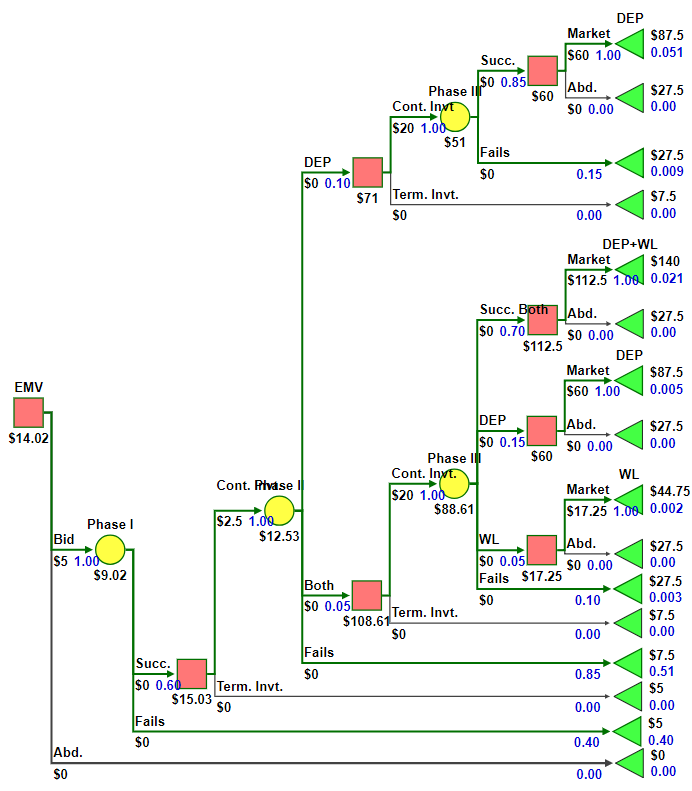
\includegraphics[width = 1.\linewidth]{bio_5_255}
\caption{BIO Decision Tree 5\% Royalty and \$225M Marketing Cost} 
\label{pharma_tree_255} 
\end{figure}

\subsection{Policy Table}
\label{sec:pol}
Table below shows the policy table extracted from the project brief with nomenclature as follows: Pre: Prerequisites, Eff: Effectiveness,  PH CF: PHARMA Cash flow, BIO CF: BIO Cash flow, Succ: Probability of success
\begin{table}[h]
\begin{tabular}{llllll}
\textbf{Phase} & \textbf{Pre.} & \textbf{Eff.} & \textbf{PH. CF. /\$M} & \textbf{BIO CF. /\$M} & \textbf{Succ. /\%} \\
I              & -                     & N/A                    & -30                                  & 5                                 & 60                               \\
II.i           & I                     & DEP             & -40                                  & 2.5                               & 10                               \\
III.i          & II.i                  & DEP             & -200                                 & 20                                & 85                               \\
III.ii         & II.ii                 & WL            & -40                                  & 2.5                               & 15                               \\
II.iii         & I                     & Both                   & -40                                  & 2.5                               & 5                                \\
III            & II.iii                & Both                   & -500                                 & 40                                & 70                               \\
III            & II.iii                & DEP             & -500                                 & 40                                & 70                               \\
III            & II.iii                & WL            & -500                                 & 40                                & 10                               \\
Market         & III                   & DEP             & 950                                  & -                                 & N/A                              \\
Market         & III                   & WL            & 245                                  & -                                 & N/A                              \\
Market         & III                   & Both                   & 1850                                 & -                                 & N/A                             
\end{tabular}
\end{table}
\ifCLASSOPTIONcaptionsoff
  \newpage
\fi

\begin{thebibliography}{1}

\bibitem{bioe}
R. Mason, N. Savva \& S. Scholtes (2008), \emph{The Economics of Licensing Contracts}, 
\hskip 1em\relax Nature Biotechnology Vol.6 No.8
	
\bibitem{coursework}
P. Markou (2018), \emph{3E3 Coursework handout} \hskip 1em\relax University of Cambridge

\end{thebibliography}

\end{document}





